\renewcommand{\thechapter}{\Roman{chapter}}  % just don't do this :)

\chapter{Quantenmechanik - Intro}

Quantenmechanik (QM) beschreibt den Mikrokosmos (im Gegensatz zum Makrokosmos).

\noindent
$ \rightarrow $ im CD-Player\\
$ \rightarrow $ im Handy\\
$ \rightarrow $ Kernspin\\
$ \rightarrow $ Zeitstandards\\
%\begin{enumerate}[$ \rightarrow $]
%	\item im CD-Player
%	\item im Handy
%	\item Kernspin
%	\item Zeitstandards
%\end{enumerate}

\noindent
QM ist ,,merkwürdig`` insofern, als anthropomorpher Anschauung unangepasst. $ \Rightarrow $ Sie sorgt noch heute für hitzige und kontroverse Debatten.

\begin{itemize}
	\item[$ \rightarrow $] siehe Podcasts PI - Kolloquium, z.B. Nicoles Gisin 15.04.2009, Reinhard Werner 24.12.2007
	\item[$ \rightarrow $] mathematischer Rahmen relativ einfach, doch Interpretation schwierig\\
	$ \Rightarrow $ Feynman: ,,Shut up and calculate{!}``
\end{itemize}
\textbf{Historische Genese:} Wie (fast?) alle physikalischen Theorien aus experimenteller Evidenz, die mit der,,klassischen`` Theorie nicht vereinbar war.\\[5pt]
Aus \textbf{theoretischer ,,Notlage`` angesichts bestehender Experimente:}\\
Balmer-Linien (1885), Franck-Hertz-Versuch (1913), Photoeffekt (Hallweds 1888 \& Einstein 1905), Schwarzkörperspektrum (Planck 1900), Compton-Effekt (1921), Kernspaltung (Halm, Meitner und Strassmann 1939), Stern-Gerlach-Versuch (1921).\par
\textbf{Große Namen:} N. Bohr, W. Heisenberg, E. Schrödinger, M. Born, John v. Neumann, A. Sommerfeld, L. de Broglie, P. Dirac, W. Pauli, L. Szil\'ard, R. Oppenheimer, Gamow, Siegelt, Hellmann, Etore Majorana.\par
Zu Majorana: Leonardo Sciascia: La Scomparsa di Majorana (Das Verschwinden des Majorana).\par
\textbf{Buchempfehlung:} Richard Rhodes: Die Atombombe oder die Geschichte des 8. Schöpfungstages\par
Weitere Quantenmechaniker: E. Teller, A. Sacharov, L. Landau, J. Belt, M. Gutzwiller.\\[10pt]

\noindent
\textbf{Korrespondenzprinzip:} Wie korrespondieren die QM-Theorien mit den klassischen Theorien? Wie sieht der Übergang vom diskreten zu einem kontinuierlichen Spektrum aus?\\[5pt]
\textbf{Beispiel:} Atommodell mit quantisierten Elektronen-Orbitalen von Bohr und dem Klassischeren Modell von Rutherford und kontinuierlichen Kepler-Orbitalen.\\
Die Energieniveaus eines Wasserstoff Atoms sind: $ E = \frac{1}{2n^2} $. Daraus folgt, dass höhere Energieniveaus immer näher aneinander liegen. Die Einergiedifferenzen $ E_{n+1} - E_{n} \sim \hbar \omega_{\tx{Kepler}} $ werden also immer geringer. Die Umlauffrequenz kann also mit zunehmender Hauptquantenzahl immer genauer bestimmbar.

% 29.04.19

\section{Wave-particle duality at the double-slit}
\label{Isection1}

% T1
\begin{figure}[h]
	\begin{tikzpicture}
	\coordinate (a) at (0,0);
	\coordinate (b) at (1.2,0);
	\coordinate (c) at (3.5,0);
	\coordinate (d) at (6,0);
	
	%a
	\filldraw[black] (a) circle (1mm);
	\foreach \c in {1.5,0.75,0,-0.75,-1.5}
	\draw (a) -- (1,\c);
	
	%b
	\draw ($(b) + (0,0.7)$) -- ($(b) + (0,2.2)$);
	\draw ($(b) + (0,0.5)$) node[right] {$S_2$} -- ($(b) + (0,-0.5)$) node[right] {$S_1$};
	\draw ($(b) + (0,-0.7)$) -- ($(b) + (0,-2.2)$);
	
	%c
	\draw ($(c) + (0,-2.2)$) -- ($(c) + (0,2.2)$);
	\draw ($(c) + (0,-2.1)$) .. controls ($(c) + (0,-1.8)$) and ($(c) + (-0.4,-1.7)$) .. ($(c) + (-0.4,-1.4)$);
	\draw ($(c) + (-0.4,-1.4)$) .. controls ($(c) + (-0.4,-1.1)$) and ($(c) + (0,-1)$) .. ($(c) + (0,-0.7)$);
	\draw ($(c) + (0,-0.7)$) .. controls ($(c) + (0,-0.4)$) and ($(c) + (-0.8,-0.3)$) .. ($(c) + (-0.8,0)$);
	\draw ($(c) + (-0.8,0)$) .. controls ($(c) + (-0.8,0.3)$) and ($(c) + (0,0.4)$) .. ($(c) + (0,0.7)$);
	\draw ($(c) + (0,2.1)$) .. controls ($(c) + (0,1.8)$) and ($(c) + (-0.4,1.7)$) .. ($(c) + (-0.4,1.4)$);
	\draw ($(c) + (-0.4,1.4)$) .. controls ($(c) + (-0.4,1.1)$) and ($(c) + (0,1)$) .. ($(c) + (0,0.7)$);
	\node[below] at ($(c) + (0,-2.1)$) {Light, Water};
	\node[below] at ($(c) + (0,-2.5)$) {etc Waves};
	
	%d
	\draw ($(d) + (0,-2.2)$) -- ($(d) + (0,2.2)$);
	\draw[red] ($(d) + (-0.8,0.5)$) .. controls ($(d) + (-0.8,0.2)$) and ($(d) + (0,0.1)$) .. ($(d) + (0,-0.5)$);
	\draw[red] ($(d) + (-0.8,0.5)$) .. controls ($(d) + (-0.8,0.8)$) and ($(d) + (0,0.9)$) .. ($(d) + (0,1.5)$);
	\draw[blue] ($(d) + (-0.8,-0.5)$) .. controls ($(d) + (-0.8,-0.2)$) and ($(d) + (0,-0.1)$) .. ($(d) + (0,0.5)$);
	\draw[blue] ($(d) + (-0.8,-0.5)$) .. controls ($(d) + (-0.8,-0.8)$) and ($(d) + (0,-0.9)$) .. ($(d) + (0,-1.5)$);
	\draw[green] ($(d) + (-0.85,-0.3)$) .. controls ($(d) + (-0.85,-0.5)$) and ($(d) + (0,-0.7)$) .. ($(d) + (0,-1.5)$);
	\draw[green] ($(d) + (-0.85,0.3)$) .. controls ($(d) + (-0.85,0.5)$) and ($(d) + (0,0.7)$) .. ($(d) + (0,1.5)$);
	\draw[green] ($(d) + (-0.85,0.3)$) .. controls ($(d) + (-0.85,0.2)$) and ($(d) + (-0.7,0.1)$) .. ($(d) + (-0.7,0)$);
	\draw[green] ($(d) + (-0.85,-0.3)$) .. controls ($(d) + (-0.85,-0.2)$) and ($(d) + (-0.7,-0.1)$) .. ($(d) + (-0.7,0)$);
	\node[right] at ($(d) + (0.5,1)$) {Red: Slit 1 closed};
	\node[right] at ($(d) + (0.5,-1)$) {Blue: Slit 2 closed};
	\node[right] at ($(d) + (0.5,0)$) {Green: Both slits open};
	\node[below] at ($(d) + (0,-2.3)$) {Tennisballs};
	\end{tikzpicture}
	\centering
	\caption{Double-slit Experiment by Young (1803)}
\end{figure}
\textbf{For Waves} the complex amplitudes $ E_1(x) $ and $ E_{2}(x) $ coming from slits 1 and 2 and arriving at point $ x $ on the screen add up
\begin{equation}
E(x) = E_1(x) + E_2(x)
\end{equation}
The corresponding intensity reads:
\begin{equation}
I(x) \propto |E(x)|^2 = \ub{|E_1(x)|^2 + |E_2(x)|^2}_{\substack{\tx{``classical'' intensities} \\ \tx{e.g. with Tennis balls} \\ \tx{\textbf{ladder} contribution} }} + \ub{2 \Re \left(E_1^{*}(x) E_2(x)\right)}_{\substack{\tx{intererence term} \\ \sim \cos (\varphi_2(x) - \varphi_1(x) ) \\ \tx{contains phase information} \\\ \tx{\textbf{cross} term}}}
\label{1 2}
\end{equation}
\begin{equation*} % T2
|E_1 + E_2|^2 = (E_1 + E_2) (E_1^* + E_2^*) = |E_1|^2 + |E_2|^2 + 2 \Re| E_1^* E_2|
\end{equation*}
\begin{figure}[h]
	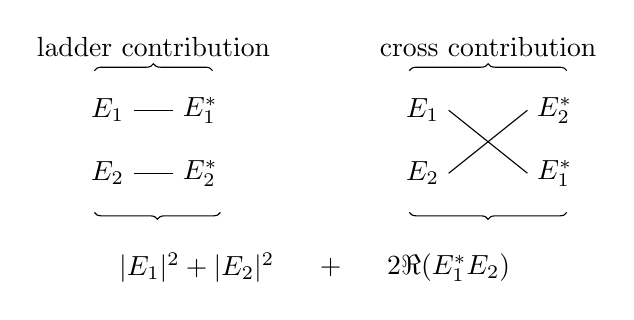
\begin{tikzpicture}[decoration=brace]
	\draw (0,0) node[left] {$E_2$} -- (0.5,0) node[right] {$E_2^*$};
	\draw (0,0.8) node[left] {$E_1$} -- (0.5,0.8) node[right] {$E_1^*$};
	\draw[decorate, yshift=2ex]  (-0.5,1) -- node[above=0.4ex] {ladder contribution}  (1,1);
	\draw[decorate, yshift=2ex]  (1.1,-0.8) -- (-0.5,-0.8);
	\node at (0.8,-1.2) {$|E_1|^2+|E_2|^2$};
	\draw (4,0) node[left] {$E_2$} -- (5,0.8) node[right] {$E_2^*$};
	\draw (4,0.8) node[left] {$E_1$} -- (5,0) node[right] {$E_1^*$};
	\draw[decorate, yshift=2ex]  (3.5,1) -- node[above=0.4ex] {cross contribution}  (5.5,1);
	\draw[decorate, yshift=2ex]  (5.5,-0.8) -- (3.5,-0.8);
	\node at (4,-1.2) {$2 \Re(E_1^*E_2)$};
	\node at (2.5,-1.2) {$+$};
	\end{tikzpicture}
	\centering
\end{figure}\\

$ \rightarrow $ \textbf{Light is a wave phenomenon}\\[10pt]
\newpage
%T3
\noindent
\begin{figure}[h]
	\begin{tikzpicture}
	\coordinate (a) at (0,0);
	\coordinate (b) at (1.2,0);
	\coordinate (c) at (3.5,0);
	\coordinate (d) at (6,0);
	
	%a
	\filldraw[gray] ($(a) + (0.5,-1.5)$) -- ($(a) + (0.86,-1.5)$) -- ($(a) + (0.8,1.5)$) -- ($(a) + (0.5,1.5)$) -- ($(a) + (0.5,-1.5)$);
	\node at ($(a) + (0.5,1.8)$) {Filter};
	\filldraw[black] (a) circle (1mm);
	\foreach \c in {1.5,0.75,0,-0.75,-1.5}
	\draw (a) -- (1,\c);
	
	%b
	\draw ($(b) + (0,0.7)$) -- ($(b) + (0,2.2)$);
	\draw ($(b) + (0,0.5)$) node[right] {$S_2$} -- ($(b) + (0,-0.5)$) node[right] {$S_1$};
	\draw ($(b) + (0,-0.7)$) -- ($(b) + (0,-2.2)$);
	
	%c
	\draw ($(c) + (0,-2.2)$) -- ($(c) + (0,2.2)$);
	\draw ($(c) + (0,-2.1)$) .. controls ($(c) + (0,-1.8)$) and ($(c) + (-0.4,-1.7)$) .. ($(c) + (-0.4,-1.4)$);
	\draw ($(c) + (-0.4,-1.4)$) .. controls ($(c) + (-0.4,-1.1)$) and ($(c) + (0,-1)$) .. ($(c) + (0,-0.7)$);
	\draw ($(c) + (0,-0.7)$) .. controls ($(c) + (0,-0.4)$) and ($(c) + (-0.8,-0.3)$) .. ($(c) + (-0.8,0)$);
	\draw ($(c) + (-0.8,0)$) .. controls ($(c) + (-0.8,0.3)$) and ($(c) + (0,0.4)$) .. ($(c) + (0,0.7)$);
	\draw ($(c) + (0,2.1)$) .. controls ($(c) + (0,1.8)$) and ($(c) + (-0.4,1.7)$) .. ($(c) + (-0.4,1.4)$);
	\draw ($(c) + (-0.4,1.4)$) .. controls ($(c) + (-0.4,1.1)$) and ($(c) + (0,1)$) .. ($(c) + (0,0.7)$);
	\node[below] at ($(c) + (0,-2.1)$) {Light, Water};
	\node[below] at ($(c) + (0,-2.5)$) {etc Waves};
	
	%d
	\draw ($(d) + (0,-2.2)$) -- ($(d) + (0,2.2)$);
	\draw[red] ($(d) + (-0.8,0.5)$) .. controls ($(d) + (-0.8,0.2)$) and ($(d) + (0,0.1)$) .. ($(d) + (0,-0.5)$);
	\draw[red] ($(d) + (-0.8,0.5)$) .. controls ($(d) + (-0.8,0.8)$) and ($(d) + (0,0.9)$) .. ($(d) + (0,1.5)$);
	\draw[blue] ($(d) + (-0.8,-0.5)$) .. controls ($(d) + (-0.8,-0.2)$) and ($(d) + (0,-0.1)$) .. ($(d) + (0,0.5)$);
	\draw[blue] ($(d) + (-0.8,-0.5)$) .. controls ($(d) + (-0.8,-0.8)$) and ($(d) + (0,-0.9)$) .. ($(d) + (0,-1.5)$);
	\draw[green] ($(d) + (-0.85,-0.3)$) .. controls ($(d) + (-0.85,-0.5)$) and ($(d) + (0,-0.7)$) .. ($(d) + (0,-1.5)$);
	\draw[green] ($(d) + (-0.85,0.3)$) .. controls ($(d) + (-0.85,0.5)$) and ($(d) + (0,0.7)$) .. ($(d) + (0,1.5)$);
	\draw[green] ($(d) + (-0.85,0.3)$) .. controls ($(d) + (-0.85,0.2)$) and ($(d) + (-0.7,0.1)$) .. ($(d) + (-0.7,0)$);
	\draw[green] ($(d) + (-0.85,-0.3)$) .. controls ($(d) + (-0.85,-0.2)$) and ($(d) + (-0.7,-0.1)$) .. ($(d) + (-0.7,0)$);
	\node[right] at ($(d) + (0.5,1)$) {Red: Slit 1 closed};
	\node[right] at ($(d) + (0.5,-1)$) {Blue: Slit 2 closed};
	\node[right] at ($(d) + (0.5,0)$) {Green: Both slits open};
	\node[below] at ($(d) + (0,-2.3)$) {Tennisballs};
	
	\end{tikzpicture}
	\centering
	\caption{T3 Doppelspalt mit Filter}
\end{figure}

\noindent
If we make the source weaker and weaker and have a sufficiently sensitive screen/detector, we observe the arrival of \textbf{single point-like} photons on the screen (photo-electric effect Einstein (1905) ($ \to $ corpusculan hypothesis))\par
By making the source sufficiently weak, we can ensure that at most 1 photon is present in the interferometer at a given time. $ \rightarrow $ no possible interaction between photons!\par
\begin{center}
	\ribox{If we \textbf{integrate} over many single detection events, we recover the interference pattern.}
\end{center}
We can make statistical predictions about the position of individual detection events (the integrated signal forms a probabilistic distribution) but the individual photons clearly don't have a deterministic trajectory (otherwise no interference).

\subsection*{Summary}

\begin{itemize}
	\item Upon detection, light behaves like an assembly of particles.
	\item The density of detection events reproduces the predictions of the wave picture (classical electromagnetism).
	\item We cannot explain the appearance of an interference pattern if we treat the photons as classical particles. Each photon goes through both slits 1 and 2: two classically exclusive alternatives.
\end{itemize}

\subsection{Consequences and terminology}

The agreement of the probability distribution for individual detections events with the predictions of optics (classical field theory) justifies referring to $ E(x,t) $ as a \textbf{probability amplitude} of the photons. $ |E(x,t)|^2 $ is the corresponding \textbf{probability density} (normalized, real, other attributes \dots) for detection at point $ x $ and time $ t $. Later on, we use $ \psi(x,t) $ instead of $ E(x,t) $ for the \textbf{wavefunction}.\par
The appearance of both wave and particle properties in the behavior of microscopic objects is known as \textbf{wave-particle duality}.\par
This raises the question of the ``\textbf{critical scale}'' below which these phenomenon take place and above which our classical representations hold.

\subsubsection*{\emph{Remarks:}}

\begin{enumerate}[I)]
	\item In optics, interference follows from the superposition principle, which is a consequence of the linearity of the field equations.\par
	Correspondingly the equations of QM are also linear and the superpositions principle applies.
	\item The probabilistic predictions of the wave picture can only be accessed by accumulating many individual detection events, i.e. by repeating the same experiment.\par
	Individual events are not predictable, QM only makes statistical predictions.
	\item These is a strong effect to push this critical scale function into the macroscopic world (e.g. experiments M. Arndt, Vienna interference of $ C_{60} $ molecules).
\end{enumerate}

\section{Measure, filtering and spectral decomposition}
\label{Isection2}

(Messung, Filterung und spektrale Zerlegung)

%T4
\noindent
\begin{figure}[h]
	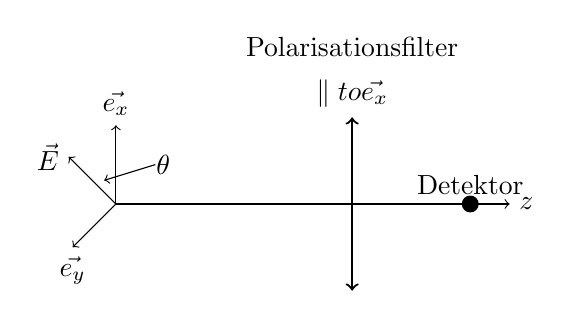
\begin{tikzpicture}
	\draw[->] (0,0) -- (5,0) node[right] {$z$};
	\draw[->] (0,0) -- (0,1) node[above] {$\vec{e_x}$};
	\draw[->] (0,0) -- (-0.55,-0.55) node[below] {$\vec{e_y}$};
	\draw[->] (0,0) -- (-0.6,0.6) node[left] {$\vec{E}$};
	\centerarc[](0,0)(90:135.5:0.5);
	\draw[->] (0.5,0.5) -- (-0.15,0.3);
	\node at (0.6,0.5) {$\theta$};
	\draw[thick,<->] (3,1.1) node[above] {$\parallel \text{ to } \vec{e_x}$} -- (3,-1.1);
	\node at (3,2) {Polarisationsfilter};
	\filldraw (4.5,0) node[above] {Detektor} circle (0.1cm);
	\end{tikzpicture}
	\centering
	\caption{Linearly polarized beam of monochromatic light}
\end{figure}
\noindent
Classical field:
\begin{equation}
\vec{E}(\vec{r},t) = E_0 \hat{e}_{p} e^{i (k z - \omega t)}
\end{equation}
\begin{align*}
\vec{E}(\vec{r},t) = \ \ & E_0 \cos \theta \vec{e}_x e^{i(kz - \omega t)}\\
+ & E_0 \sin \theta \vec{e}_{y} e^{i(kz - \omega t)}
\end{align*}
After the filter
$$ \vec{E}(\vec{r},t) = E_0 \cos\theta \vec{e}_{x}e^{i(kz - \omega t)} $$
Intensity:
\begin{equation*}
I' \propto | E' |^2 \qquad I \propto | E | ^2
\end{equation*}
\frbox{Malus' law}{
\begin{equation}
I' = I \cos^2 \theta
\label{Malus}
\end{equation}}
\noindent
What happens if we weaken the source to obtain single photons?\\
$ \rightarrow $ 2 possible options:
\begin{itemize}
	\item a single photons passes completely (click on detector): event ``1''
	\item or it does not pass at all (no click): event ``0''
\end{itemize}
For each photon, the outcome cannot be predicted with certainty.\par
Upon averaging over a large number of photons, the fraction which makes it through is:
\begin{equation*}
\frac{N_1}{n_1 + n_0} \to \cos^2 \theta
\end{equation*}
in accordance with Malus' law \eqref{Malus}.\\[10pt]
E.g.: \texttt{10010001110101}\\[5pt]
Special casses:
\begin{itemize}
	\item $ \theta = \phantom{0}0^\circ \quad \to $ all photons go through: $\phantom{1}$\texttt{1111\dots1}
	\item $ \theta = 90^\circ \quad \to $ no photon goes through: \texttt{0000\dots0}
\end{itemize}
$ \Rightarrow $ in this case the output is certain but experiment must be repeated many times to prove that this is the case.\\[10pt]
In these cases, we say that the photon finds itself in an \textbf{eigenstate}. One state: $ |1\rangle $ for $ \hat{e}_x $ polarized and one state $ |0\rangle $ for $ \hat{e}_y $ polarized which is associated with the particular outcomes for \textbf{eigenvalues} 1 and 0.\\[10pt]

% 30.04.19

\noindent
Sichere (Quanten-) Ereignisse gibt es allein für $ \hat{e}_p = \hat{e}_x $ bzw. $ \hat{e}_p = \hat{e}_y $. Diese Polarisationsrichtungen definieren die \textbf{Eigenzustände} $ |1\rangle \ (\hat{e}_x) $ bzw. $ |0\rangle \ (\hat{e}_y) $ zu den \textbf{Eigenwerten} 1 bzw. 0.\\[10pt]
Für eine allgemeine Wahl von $ \hat{e}_p $ haben wir die Orthogonalzerlegung 
\begin{equation}
\hat{e}_p = \hat{e}_x \cos\theta + \hat{e}_y \sin 
\theta
\label{spektrale zerlegung}
\end{equation}
Die Wahrscheinlichkeit für ,,0`` \textbf{oder} ,,1`` ergibt sich als:,
\begin{equation}
\cos^2 \theta + \sin^2 \theta = 1
\label{cos2sin2}
\end{equation}
wie gewünscht.\par
\eqref{spektrale zerlegung} kann als ,,\textbf{spektrale Zerlegung}`` des Polarisationszustandes $ \hat{e}_p $ in die durch den Messapparat/Filter definierten Eigenzustände $ \hat{e}_x $ und $ \hat{e}_y $ bzw. $ |1\rangle $ und $ |0\rangle $.\par
Lässt man Photonen, die durch $ F $ transmittiert werden, durch einen weiteren Filter $ F' $ der selben Orientierung wie $ F $ gehen, so folgt ein \textbf{sicheres} Ereignis, da das Photon durch $ F $ im Eigenzustand $ \hat{e}_x $ von $ F' $ \textbf{präpariert} wurde.\par
In diesem Sinne: Zustandspräparation $ \equiv $ Filterung (-smessung)

\subsubsection*{\emph{Bemerkung}}

\begin{enumerate}[(1)]
	\item Um sich davon zu überzeugen, dass das System in einem Eigenzustand präpariert wurde, muss Statistik über viele ($ N \gg 1 $) Photonen betrieben werden.
	\item \eqref{spektrale zerlegung} und \eqref{cos2sin2} legen bereits de essentielle Vektorraumstruktur des QM mit vorzugsweise orthonormierten Basisvektoren fest.
	\item Systeme, die sich mit $ |0\rangle $ und $ |1\rangle $ vollständig beschreiben lassen heißen: \textbf{Zweiniveausysteme}
\end{enumerate}

% 6.05.19

